\documentclass[a4paper,10pt,oneside]{article}
\usepackage{graphicx}
\usepackage{color}
\usepackage{url}
\usepackage{subfigure}
\usepackage[utf8]{inputenc}
\usepackage[T1]{fontenc}
\usepackage{tgpagella}
%\usepackage[scale=0.9]{tgcursor}
%\usepackage[scale=0.9]{tgheros}
\usepackage{xstring}

\newcommand{\myscale}{0.74}
\newcommand{\vect}[1]{\boldsymbol{#1}}
\newcommand{\punts}[1]{\StrSubstitute{#1}{.}{.\.}}
\newcommand{\code}[1]{\texttt{\StrSubstitute{#1}{.}{.\.}}}
\def\.{\discretionary{}{}{}}
\newcommand{\jmodule}[1]{\texttt{\textit{#1}}}

\setlength{\hoffset}{-1in} %left margin will be 0, as hoffset is by default 1inch
\setlength{\voffset}{-1in} %analogous voffset
\setlength{\oddsidemargin}{1.5cm}
\setlength{\evensidemargin}{1.5cm}
\setlength{\topmargin}{1.5cm}
\setlength{\textheight}{24cm}
\setlength{\textwidth}{18cm}

\def\mftitle{jInfer BasicIGG Module Description}
\def\mfauthor{Michal Klempa, Mário Mikula, Robert Smetana, Michal Švirec, Matej Vitásek}
\def\mfadvisor{RNDr. Irena Mlýnková, Ph.D., Martin Nečaský, Ph.D.}
\def\mfplacedate{Praha, 2011}
\title{\bf\mftitle}
\author{\mfauthor \\ Advisors: \mfadvisor}
\date{\mfplacedate}

\ifx\pdfoutput\undefined\relax\else\pdfinfo{ /Title (\mftitle) /Author (\mfauthor) /Creator (PDFLaTeX) } \fi

\begin{document}
\maketitle
\noindent Target audience: developers willing to extend jInfer, specifically modify the way \jmodule{BasicIGG} creates initial grammar from input files, for example by adding support for a new schema language.

\noindent \begin{tabular}{|l|l|} \hline
Responsible developer: & Matej Vitásek \\ \hline
Required tokens:       & none \\ \hline
Provided tokens:       & cz.cuni.mff.ksi.jinfer.base.interfaces.inference.IGGenerator \\ \hline
Module dependencies:   & Base \\ \hline
Public packages:       & cz.cuni.mff.ksi.jinfer.basicigg.properties \\ \hline
\end{tabular}

\section{Introduction}

This is an extensible implementation of the \jmodule{IGGenerator} inference interface. It is the only IG generator officialy shipped with jInfer.\\
Make sure you understand the difference between the two types of initial grammar as described in \cite{archdoc}.

\section{Structure}

The main class implementing \code{IGGenerator} inference interface and simultaneously registered as its service provider is \code{IGGeneratorImpl}. In its \code{start} method it enumerates all files in the input parameter (of type \code{Input}). For each file, based on its extension the correct \emph{processor} is selected, executed and returned rules are aggregated. After each file has been processed, the resulting grammar is returned by invoking the \code{finished} method of the callback argument. This process is illustrated in fig. \ref{figure-process}.

\begin{figure}
	\centering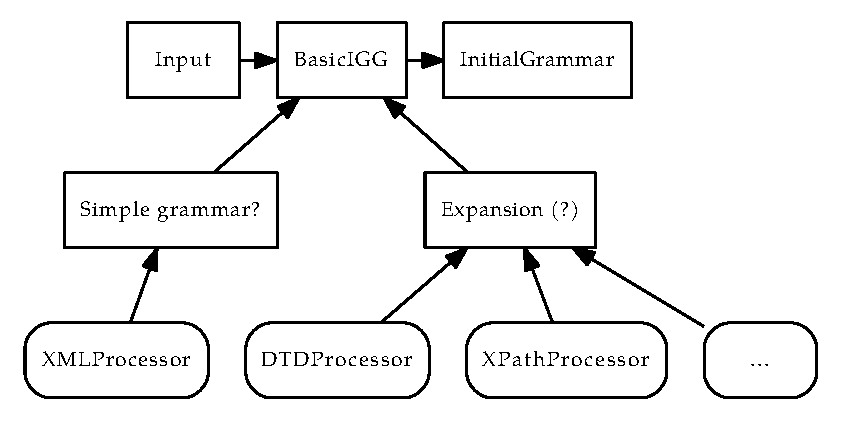
\includegraphics[scale=\myscale]{process-view}
	\caption{Process view of BasicIGG} \label{figure-process}
\end{figure}

\section{Processors}

A \emph{processor} is a class capable of extracting IG from an arbitrary \code{InputStream} (usually encapsulating a file). Various processors may handle generic XML, schemas like DTD, XSD or Schematron, query languages such as XPath, and so on.\\
A processor has to be registered as a service provider of the \code{Processor} interface from \jmodule{Base} module. Due to the nature of NBP lookups, each processor is internally kept as a singleton, and should not use its inner state (refer to the chapter Lookups in \cite{archdoc}). Note that the factory pattern is not used here (see \cite[Factory]{archdoc}).\\ % TODO anti reference to a chapter number when factory pattern is moved to arch
Each processor declares the class of inputs (documents, schemas, queries) and file extensions it is able to handle by implementing methods \code{getFolder()}, \code{getExtension()} and \code{processUndefined()}. Refer to JavaDoc of these methods for further details.\\

\jmodule{BasicIGG} comes bundled with 3 processors: for generic XML documents, DTD schemas and XPath queries. Support for XSD queries is implemented in \jmodule{XSDImporter} to demonstrate \jmodule{BasicIGG}'s extension capabilities.

\subsection{XML processor}

XML processor registers itself into \emph{document} input folder, \emph{xml} file extension and declares that it can process other arbitrary file extensions.\\
SAX traversal is used to collect the rules; the relevant \code{ContentHandler} is the class \code{TrivialHandler}. The way it works is following: every time a start of an element is encountered, a new \code{Element} is created along with its attributes. This new element representation is then placed on the top of a stack. Every other element or simple data found until its ending tag is created and attached to its subnodes. When an end of an element is encountered, the element currently on the top of the stack is closed and declared to be a rule of the IG.\\
After reaching the end of the document, all IG rules are returned. Note that this approach creates "simple" initial grammar.

\subsection{DTD processor}

DTD processor registers itself into \emph{schema} input folder, \emph{dtd} file extension and declares it cannot handle other file extensions.\\
To parse DTD files a 3rd party library is used: \jmodule{dtdparser} (\cite{dtdparser}).
Translation from the object model in this library to our own is handled mostly by \code{DTD2RETranslator} class.\\
Note that the initial grammar generated in this way is complex. Therefore, this processor checks for the \code{CAN\_\.HANDLE\_\.COMPLEX\_\.REGEXPS} capability of the simplifier following this IG generator: in positive case it simply returns the grammar, if the following module cannot handle complex regular expressions, DTD processor first invokes an \emph{Expander} (see \ref{section-expansion}).

\subsection{XPath processor}

This is a rather na\"{i}ve implementation of an XPath processor. It registers itself into \emph{query} input folder, \emph{xpath} file extension (text file containing one XPath query per line) and declares it cannot handle other file extensions.\\
To parse XPath queries, standard support present in JDK is used. The relevant \code{XPathHandler} is the \code{XPathHandler} class.\\
% TODO vektor Explain how it works...

\section{Expansion} \label{section-expansion}

Expansion is used to convert complex regular expressions in initial grammar to simple ones (concatenations of tokens) for simplifiers that can handle only the simple form. The process can be seen as breaking down a regular expression into a set of words (positive examples) that are described by this regexp. Relevant interface encapsulating any implementation of such an expander is \code{Expander} in \jmodule{Base}. Reference implementation is \code{ExpanderImpl} in this module. Note that even though this implementation is retrieved using lookups, jInfer bundles only one such implementation and does not support choice among more of them. Anyone wishing to implement his own expander will thus have to either remove jInfer's implementation, or implement the usual module selection. % TODO vektor Is this documented somewhere? anti: NO, should be in developer doc with preferences panel and so on!!!

\subsection{ExpanderImpl internals}

\code{ExpanderImpl} works recursively, and it will probably be the best to explain it from bottom to up.\\

At this point, let's denote a \emph{word} over an \emph{alphabet} typed (in Java generics sense) \emph{T} as a \code{List<T>}. Following the same logic, let's denote a set of such words as \code{List<List<T>{}>}. Our aim while expanding will be to convert a regular expression representing some node's subnodes to a list of words that are described by this regexp. In this case, \emph{T} will be \code{AbstractStructuralNode}.\\

The first interesting function is \code{ExpansionHelper.applyInterval()}. It takes a list of words extracted from a regexp (thus in the List<List<AbstractStructuralNode>{}> form) and a \code{RegexpInterval} and creates a new list of words: applying the interval on each of the words in a heuristic sense. The behaviour depends on the type of the interval.
\begin{itemize}
	\item \emph{Once}: the resulting set of words is exactly the original set of words.
	\item \emph{Optional}: same as above, but an empty word is added to the resulting set (each word from input \emph{may} or \emph{may not} occur - but one empty word is enough).
	\item \emph{General interval}: has a minimum and a maximum number of occurences. Theoretically, all counts in interval $ [min, max] $ should be considered, but for practical reasons the following heuristic is employed: each word from the input is duplicated\footnote{Duplicating a word $abc$ $N$ times results in a word $\underbrace{abcabc\ldots abc}_{N\times}$.} first $min$, then $max$ times and added to the result.
	\item \emph{Kleene star}: similar to the general interval and \emph{optional}, the result contains an empty word. Then for each word on input: this word and its 3$\times$ duplication is added to the result. Obviously, this is a heuristic approach again - theoretically each word should be duplicated between 0 and $\infty$ times in the result.
	\item \emph{Kleene cross}: except for not including empty word, this is the same case as \emph{Kleene star}: each input word is duplicated 1 and 3 times in the result.
\end{itemize}

Understanding how intervals affect the expansion, it is time to move a level up: how a regular expression is expanded. This is done in \code{ExpanderImpl.unpackRE()} performing a recursive descent into the regexp tree and returning a set of words. Based on the regexp type, one of the following is performed.
\begin{itemize}
	\item \emph{LAMBDA}: resulting word set contains one empty word.
	\item \emph{TOKEN}: resulting set contains a word with one letter: the content (an \code{AbstractStructuralNode}) of this token; the interval of the regexp is applied on this word before returning it.
	\item \emph{ALTERNATION}: first, all children of this alternation are recursively evaluated. Their respective words are appended in a list, this list has the regexp interval applied and is returned. Reasoning is the following: we are trying to get all the words a regexp can produce. If the regexp is an alternation, any word that can be produced by one of its children can be a word produced by the regexp itself.
	\item \emph{PERMUTATION}: a heuristic is applied again: because there are $n!$ ways to order children of a permutation, only two are actually picked: the original order in which they appear, and reversal of this order. In both cases the children are treated as if they we concatenation (and thus the following case is invoked) and appended in a list. On this list the regexp interval is applied and the list is returned.
	\item \emph{CONCATENATION}: this is by far the most complicated case. Let's denote word sets produced by the $N$ children of the concatenation $ w_1 \ldots w_N $. Now, all words that could be produced by this concatenations correspond to concatenations of form $w_{a_1} w_{a_2} \ldots w_{a_N}$ for all possible combinations of indices $a_i, i  \in \{1 \ldots N\}$. Number of such words grows exponentially with $N$, therefore a heuristic approach has to be employed again.\newline
In this case, consider $ m = \max_{i \in 1 \ldots N}{|w_i|} $. Now, $ m $ words will be constructed in the following way: in a for-loop enumerating $ i \in \{1 \ldots m\}$ the $j$-th part of this $i$-th word will be $w_{i mod |w_j|}$. The method \code{ExpanderImp.unpackConcat()} illustrates this.
\end{itemize}

Now for the next part, description of \code{Element} expansion. This is the content of \code{ExpanderImpl.expandElement()} method. First, element's subnodes are expanded as a regexp. For each word from this expansion a new \code{Element} is created: letters of this word are encapsulated in tokens, these tokens are put in a concatenation that constitutes subnodes of this new element. If the letter is an element itself, it is not recursively expanded - it is just declared to be a sentinel (see \cite[section 3.3]{archdoc}).\\

Finally, expanding a grammar means expanding each of its rules (elements) and returning the gathered rules (elements).

\section{Preferences}

All settings provided by \jmodule{BasicIGG} are project-wide, the preferences panel is in \code{cz.cuni.mff.ksi.jinfer.basicigg.properties} package. It is possible to set the following flags. 
\begin{itemize}
	\item Flag to keep values of attributes found in XML documents - unchecking this saves memory during the inference process, but loses all information about the attribute domain, which can lead to less expressive schema.
	\item Flag to keep simple data values from XML documents - again, unchecking saves memory (potentially a lot, with input files containing a lot of text). Drawback might again be losing information that could be useful in schema generation.
	\item Flag to stop on errors: if this flag is set, \jmodule{BasicIGG} will interrupt the inference if it comes across an error while extracting IG. Unsetting this flag allows \jmodule{BasicIGG} to ignore these errors and retrieve as much IG as possible.
\end{itemize}

\section{Data flow}

Flow of data in this module is following.
\begin{enumerate}
	\item IGGeneratorImpl walks over input files in a loop.
	\item Each file gets processed by a processor based on its folder and extension.
	\item Rules from all files are gathered in a single list (IG) and returned via a callback.
\end{enumerate}

\section{Extensibility}

\jmodule{BasicIGG} can be easily extended to support a new input type: just create a class implementing \code{Processor}, annotate it as a service provider and implement any logic needed. \jmodule{XSDImporter} is an example of this.\\

It is possible to replace the default \code{Expander} implementation: but as mentioned in \ref{section-expansion}, either the old implementation must be removed or module selection must be introduced.

\nocite{*}
\newpage
\bibliographystyle{alpha}
\bibliography{literature}

\end{document}
